\chapter{Simulation der Systemeigenschaften}
\label{chap4}
Ziel dieser Arbeit soll der Vergleich verschiedener Kombinationen von Ladesystem und Speichertechnologie aus technischer Sicht sein. Qualitative Bewertungen einer Kombination sind teilweise ohne Rechnung möglich (z. B. "`Das \textsc{primove}-Ladesystem ist besser für Lithium-Titanat-Batterien geeignet als für Lithium-Eisenphosphat-Batterien"'). Eine genauere Betrachtung und ein Vergleich von ähnlichen Technologiekombinationen ist jedoch nicht möglich. Daher werden in dieser Arbeit mit Hilfe eines Simulationsmodell quantitative Daten zu den verschiedenen Technologiekombinationen ermittelt.

\section{Simulationsmodell}
%TODO: Ausfüllen
Ausgangspunkt ist ein Elektrobus-Simulationsmodell, das im Fachgebiet Methoden der Produktenwticklung und Mechatronik der TU Berlin entwickelt wurde. Es wurde im Rahmen einer Diplomarbeit von Maximilian Götz erstellt~\cite{Gotz:2013}. Das Modell ist in \textsc{Matlab} und \textsc{simulink} programmiert. Das Modell wird kontinuierlich weiterentwickelt. Für diese Arbeit wurde die Version verwendet, die Tu-Anh Ly (MPM, TU Berlin) am 11. Juni 2015 zur Verfügung stellte. In Abbildung \ref{abb_simmodell} sind die einzelnen Komponenten des Simulationsmodells und ihre Zusammenhänge dargestellt.
\begin{figure}\centering
	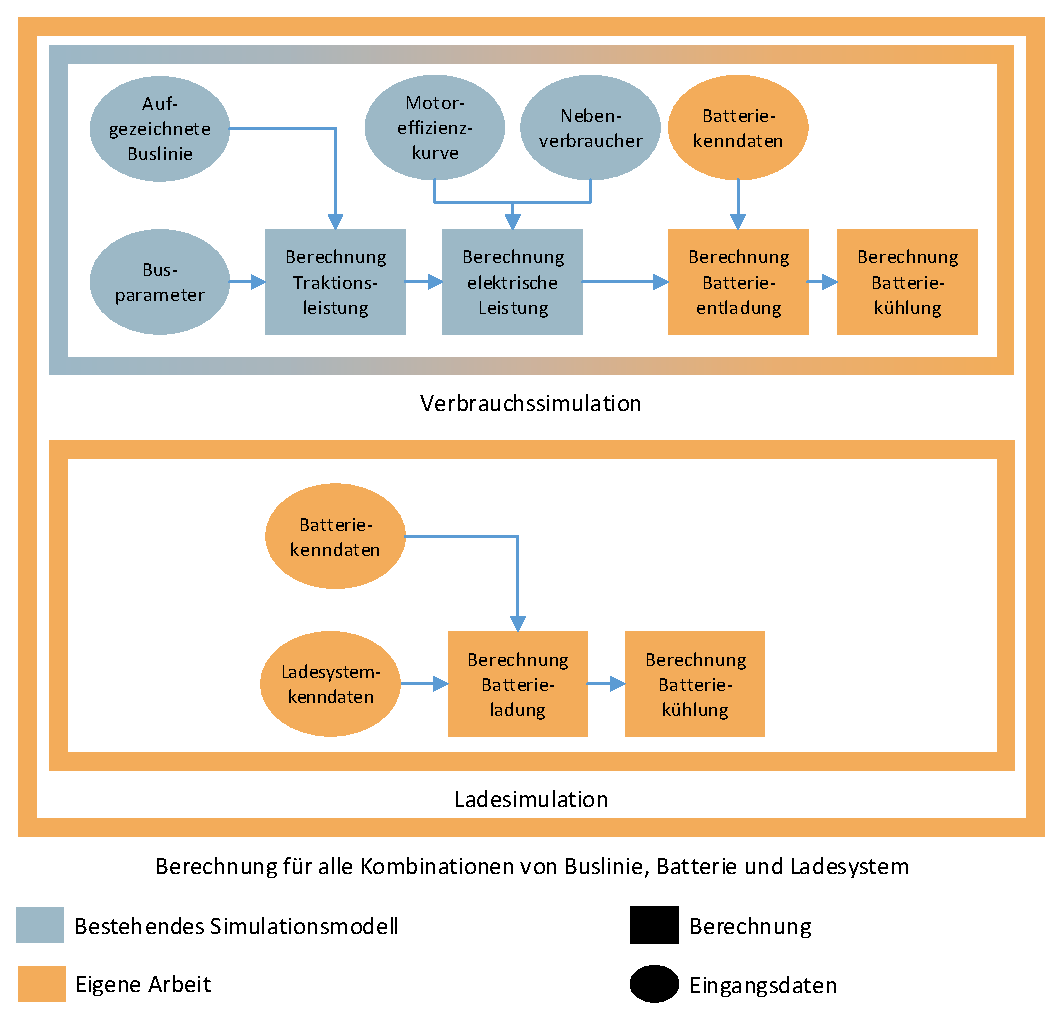
\includegraphics[width=\myFigureWideWidth]{Simulation-Schaubild}
	\caption{Komponenten des Simulationsmodells}
	\label{abb_simmodell}
\end{figure}

\paragraph{Digitaler Anhang} In Anhang \ref{an_Digital} ist eine Kopie des kompletten Simulationsmodells enthalten. Durch Ausführen von \texttt{Simulationsmodell/Batteriesimulation\_Heide.m} können die Ergebnisse reproduziert werden.

\subsection{Aufgezeichnete Strecke}
Der Energieverbrauch wird anhand einer im normalen Linienverkehr aufgezeichneten Strecke berechnet. Für jeweils einen bestimmten Umlauf wurden dabei Geschwindigkeit, Höhe über dem Meeresspiegel und Passagierzahl mit einer zeitlichen Auflösung von einer Sekunde aufgezeichnet. Es werden die Buslinien 204 und 192 der Berliner Verkehrsbetriebe (BVG) betrachtet.

Die Buslinie 204 führt vom Bahnhof Zoo zum Südkreuz. Ein Umlauf ist 12,8 km lang un dauert ca. 80 Minuten. Sie ist eine innerstädtische Linie mit niedriger Durchschnittsgeschwindigkeit und vielen Beschleunigungs- und Bremsvorgängen. Das Geschwindigkeitsprofil ist in Abbildung \ref{Abb_204} zu sehen.
\begin{figure}\centering
	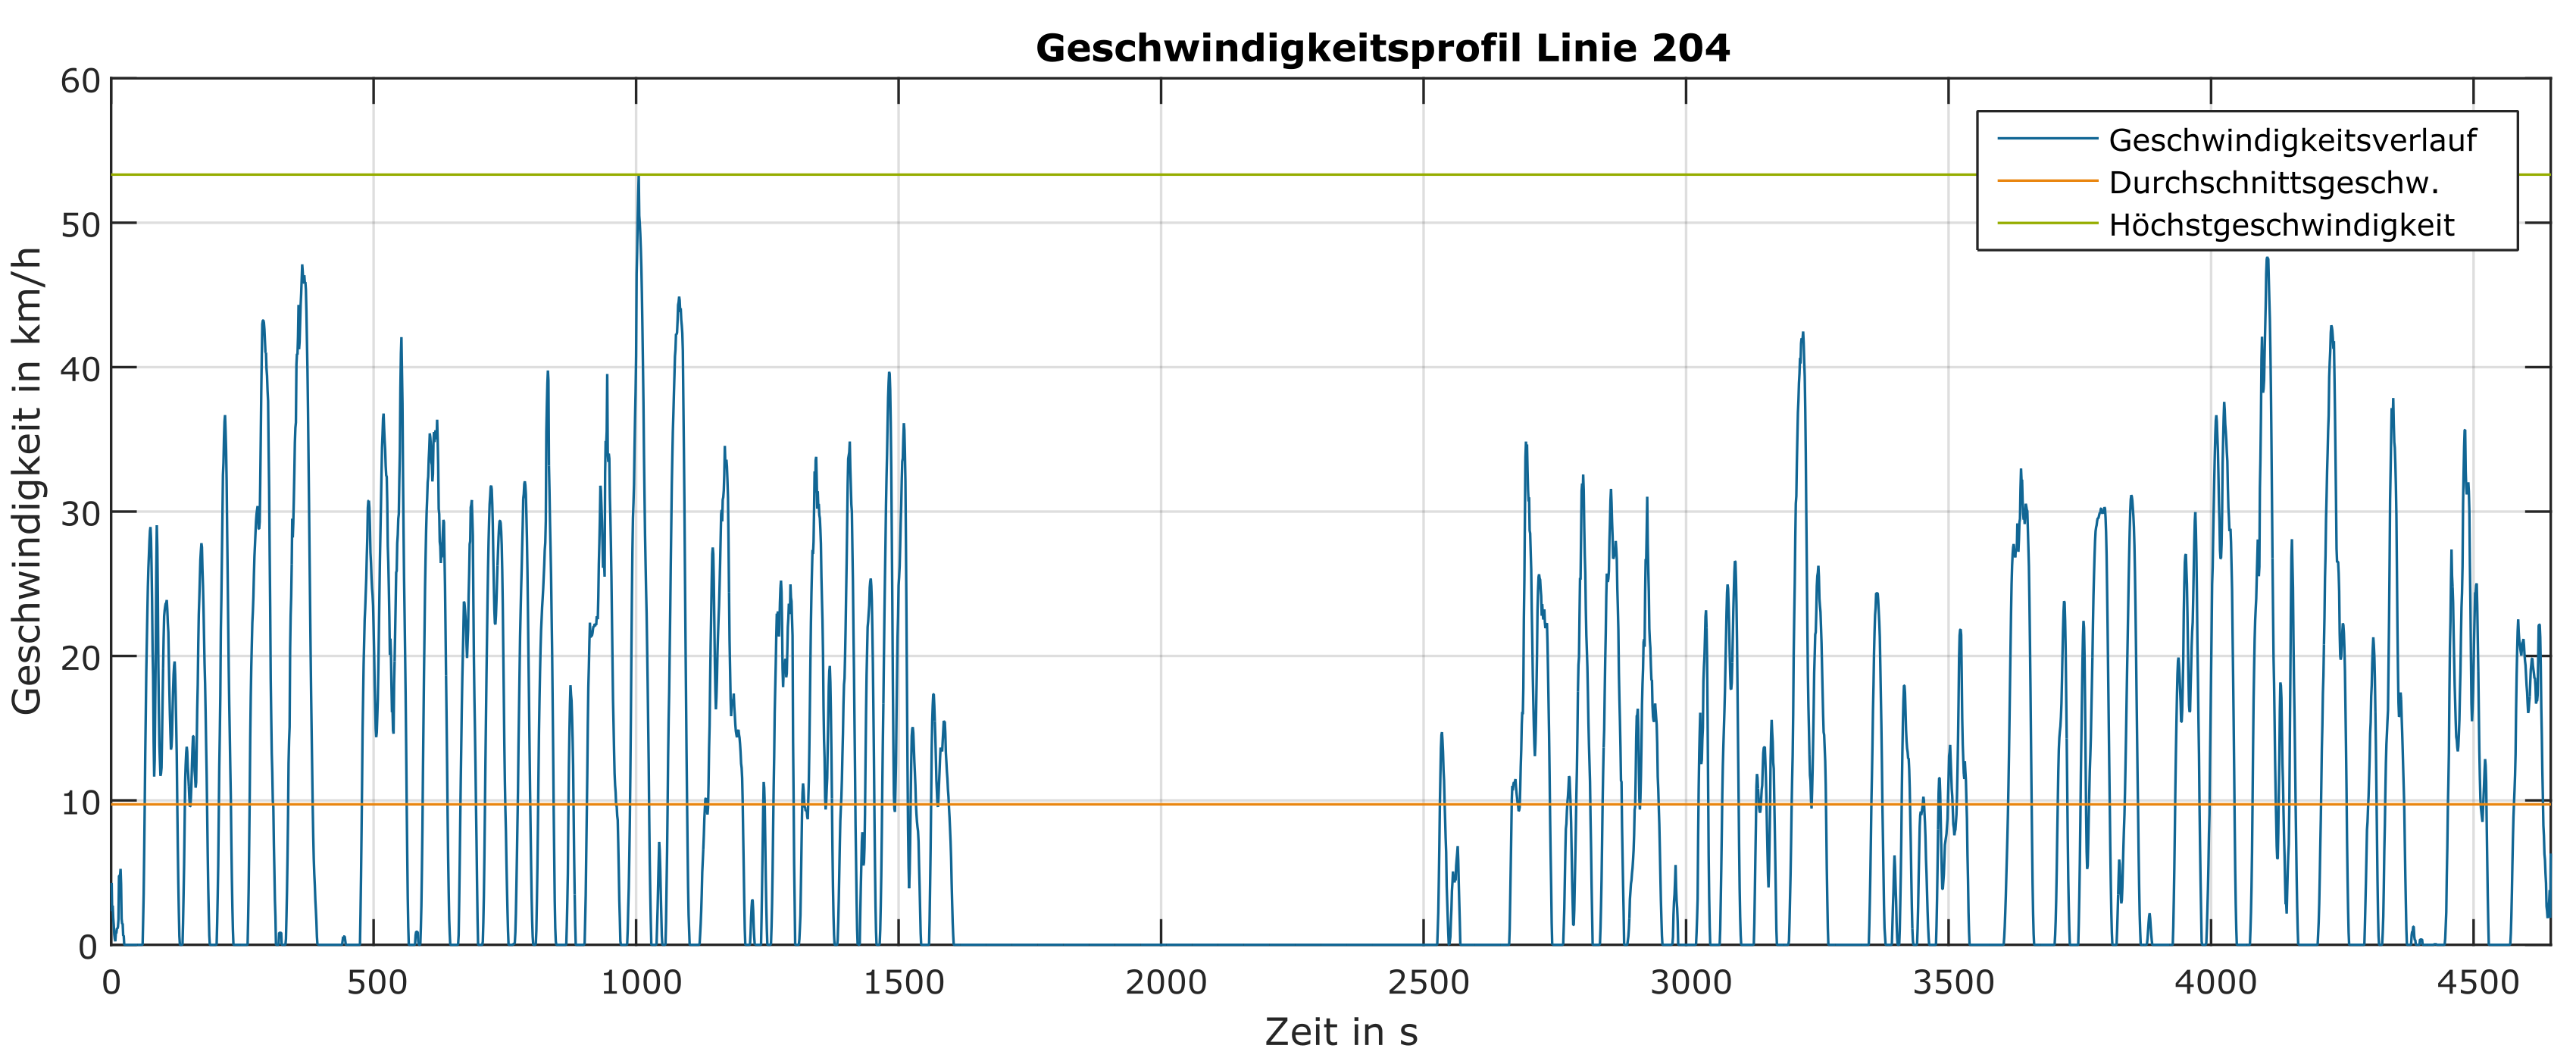
\includegraphics[width=\myFigureWideWidth]{Profil204}
	\caption{Geschwindigkeitsprofil der Buslinie 204}
	\label{Abb_204}
\end{figure}

Die Linie 192 führt vom S-Bahnhof Marzahn zum S-Bahnhof Friedrichsfelde durch den Stadtrand Berlins. Ein Umlauf ist 19,8 km lang und dauert ca. eine Stunde. Wie in Abbildung \ref{Abb_192} erkennbar ist die Durchschnittsgeschwindigkeit höher und das Geschwindigkeitsprofil gleichmäßiger.

\begin{figure}\centering
	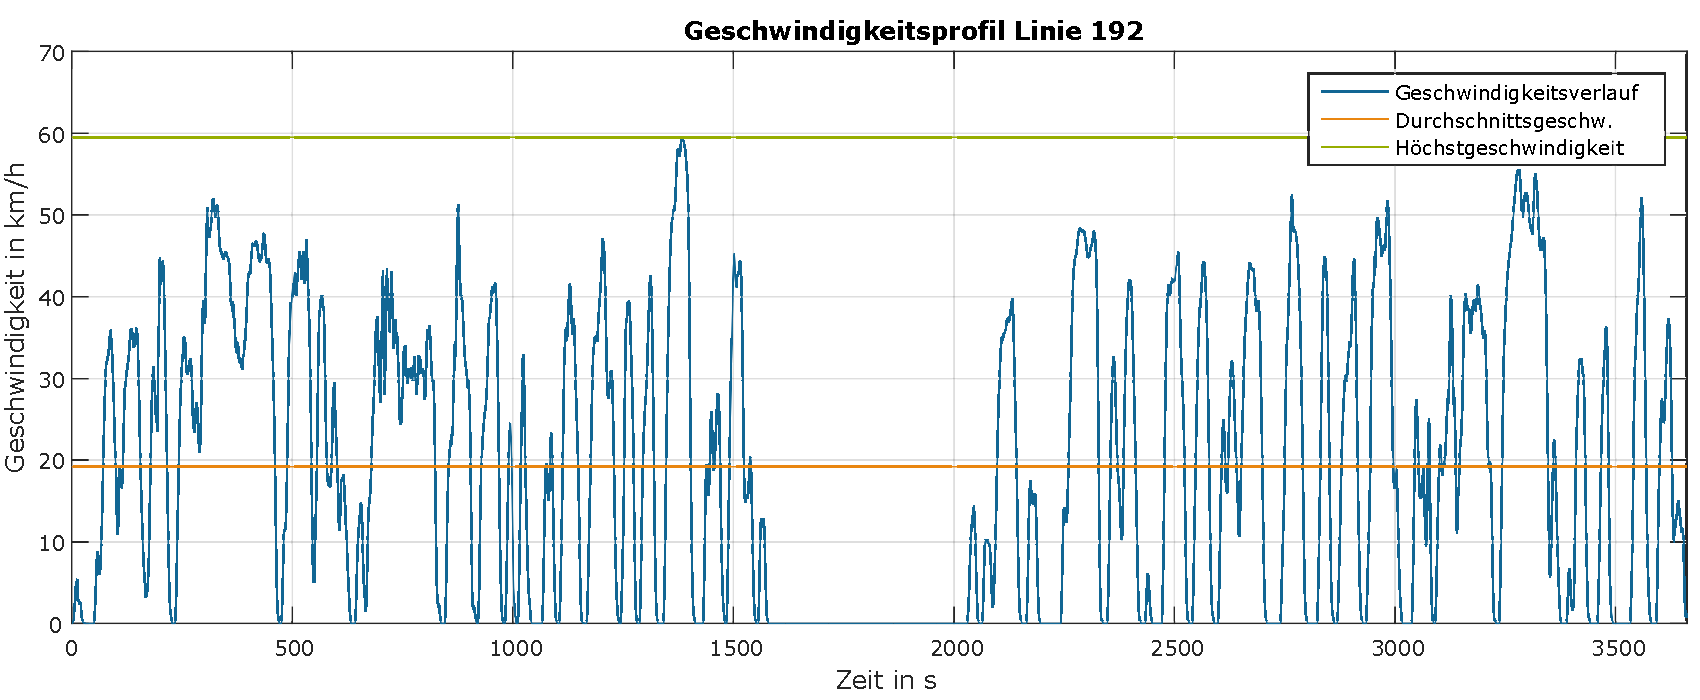
\includegraphics[width=\myFigureWideWidth]{Profil192}
	\caption{Geschwindigkeitsprofil der Buslinie 192}
	\label{Abb_192}
\end{figure}

\subsection{Energieverbrauch}
Über die aufgezeichnete Strecke sind Beschleunigung, Geschwindgkeit und Steigung zu jedem Zeitpunkt festgelegt. Mit den Busparametern Gewicht, Rollwiderstand, Stirnfläche und $c_w$-Wert werden nun die mechanischen und aerodynamischen Kräfte berechnet, die auf den Bus wirken. Aus diesen Kräften wird die erforderliche Traktionsleistung und Motordrehzahl berechnet.

%TODO: Ausfüllen
Eine von \textbf{xxx} ertellte Effizienzkurve\marginpar{Wer, Quellenvermerk!} berechnet aus Traktionsleistung und Geschwindigkeit die erforderliche elektrische Leistung. In Abbildung \ref{abb_Leistungen} werden die berechneten Leistungen für ein einfaches Geschwindigkeitsprofil gezeigt. Wie in der Abbildung zu sehen, sinkt die Effizienz des Motors mit steigender Leistung. Beim Bremsen kann der Motor als Generator betrieben werden und die Bewegungsenergie wieder in elektrische Energie umwandeln. Nur bei sehr niedrigen Geschwindigkeiten kann nicht rekuperiert werden.
\begin{figure}\centering
	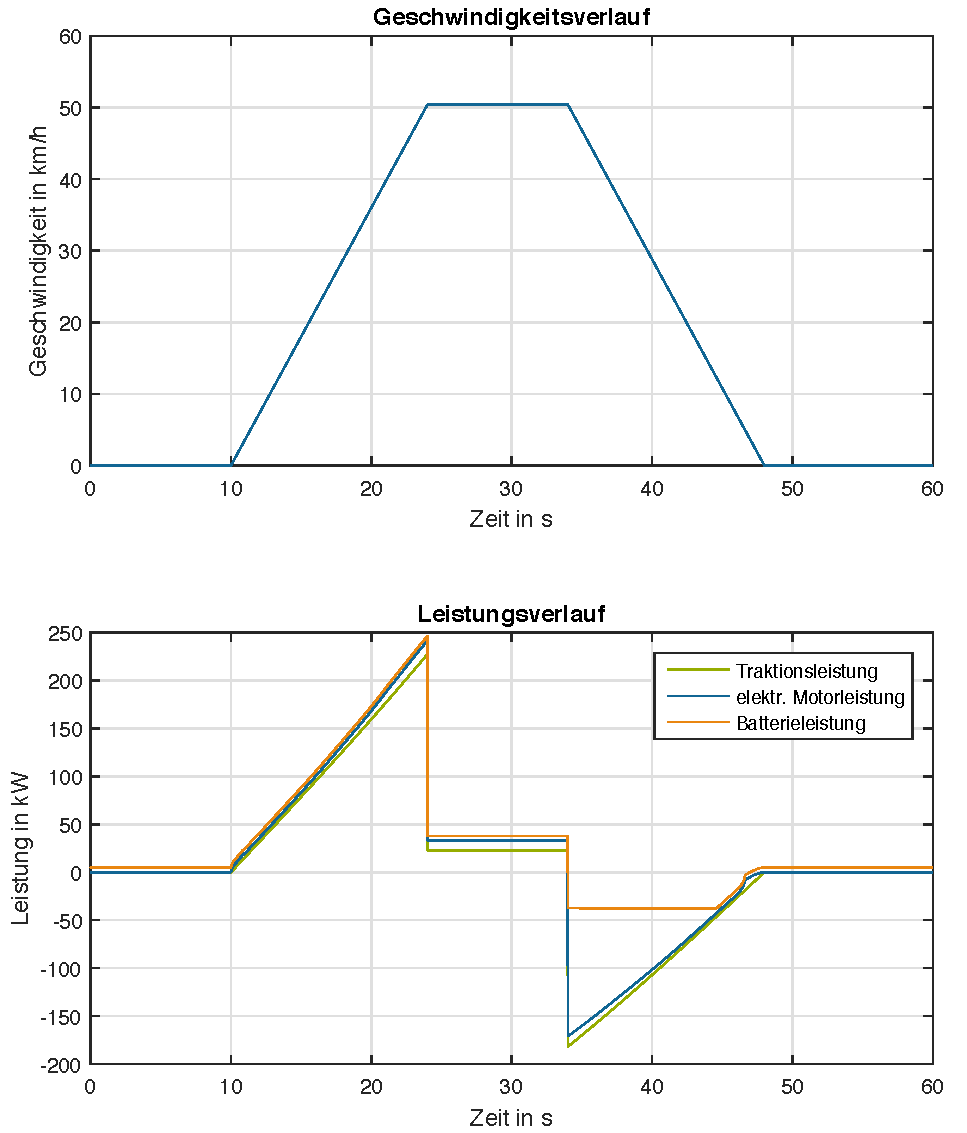
\includegraphics[width=\myFigureWideWidth]{Leistungen}
	\caption[Traktions-, Motor- und Batterieleistung]{Traktions-, Motor- und Batterieleistung für ein einfaches Geschwindigkeitsprofil. Ein Bus mit einer Masse von 13,3 Tonnen wird konstant mit 1 $\frac{m}{s^2}$ auf 50,4 $\frac{km}{h}$ beschleunigt und nach wenigen Sekunden mit 1 $\frac{m}{s^2}$ bis zum Stillstand abgebremst. Als Batterie wurde hier eine $LiFePO_4$-Batterie gewählt. Durch die maximale Ladeleistung von 38 kW kann die verfügbare Rekuperationsleistung nur begrenzt ausgenutzt werden.}
	\label{abb_Leistungen}
\end{figure}

\subsubsection{Nebenverbraucher}
Neben dem Antrieb entfällt ein signifikanter Teil der Batterieleistung auf die sogenannten Nebenverbraucher. Der weitaus wichtigste Nebenverbraucher ist die Klimatisierung des Busses. Die Kühlung erfolgt durch eine elektrische Klimaanlage mit einer maximalen Dauerleistung von 3 kW an heißen Tagen.

Für die Heizung kann nicht wie bei Dieselbussen die Abwärme des Motors benutzt werden, da der Elektromotor dafür viel zu effizient ist. Im Berliner Elektrobus sollte ursprünglich eine Wärmepumpe verwendet werden. Damit kann mehr Wärme in den Bus transportiert werden als elektrische Energie aufgewandt wird. Aufgrund von mangelnder Zuverlässigkeit wird aktuell eine direkte Heizung mit einer Leistung von durchschnittlich 10 kW an kalten Tagen verwendet. Es ist aber damit zu rechnen, das neue Elektrobusse eine Wärmepumpe zur Heizung verwenden werden. Daher wurde die Heiz- und Kühlleistung mit 3 kW abgeschätzt.

Für die anderen Nebenverbraucher wie Licht, Türen und Druckluft wird eine durchschnittliche Leistung von insgesamt 2 kW veranschlagt.

\subsection{Batteriemodell}
Da der Stromverbrauch durch die elektrische Motorleistung und die Nebenverbraucher festgelegt ist, \emph{muss} die Batterie die geforderte Fahrleistung liefern. Sie \emph{kann} bis zu ihrer maximalen Ladeleistung Rekuperationsleistung zum Aufladen nutzen. Darüber hinaus anfallende Bremsenergie wird in der Realität über einen Bremswiderstand auf dem Dach abgeleitet, daher kann sie in der Simulation ignoriert werden.

In dieser Arbeit wird das empirische Batteriemodell von Tremblay und Dessaint verwendet \cite{tremblay2009experimental}. Dieses generische Batteriemodell liefert weniger exakte Daten als spezialisierte Modelle, kann aber dafür verschiedene Batterietypen darstellen. Ein großer Vorteil dieses Modells ist, das sich die erforderlichen Parameter aus den Datenblättern der Batterien ablesen lassen. Damit kann man das Modell verschiedenen Batterietypen anpassen, ohne die Batterien selbst experimentell zu vermessen.

In Abbildung \ref{abb_Leistungen} ist neben Traktions- und Motorleistung auch die Batterieleistung aufgeführt. Im Vergleich zur maximalen Motorleistung von hier 250 kW ist die Leistung der Nebenverbraucher von 5 kW fast nicht zu sehen. Im tatsächlichen Betrieb fällt die Leistung der Nabenverbraucher permanent an, die maximale Motorleistung wird jedoch sehr selten gefordert. Daher ist der tatsächliche Anteil der Nebenverbraucher am Energieverbrauch in der Praxis größer als in einfachen Beispielen wie in Abbildung \ref{abb_Leistungen}. Die begrenzte Rekuperationsfähigkeit der Batterie zu ist in der Abbildung deutlich zu sehen.

\subsubsection{Dimensionierung}

Die simulierte Batterie ist aus mehreren Zellen zusammengesetzt. In dieser Arbeit soll die Größe der jeweils kleinsten Batterie ermittelt werden, mit der eine Fahrstrecke innerhalb von gegeben Ladezustandsgrenzen durchfahren werden kann. Aufgrund der unterschiedlichen Masse und Rekuperationsleistung verschieden großer Batterien hängt der Energieverbrauch von der Batteriegröße ab. Daher kann die optimale Batteriegröße nicht direkt aus dem Energieverbrauch mit einer Standardbatterie berechnet werden, sondern muss iterativ ermittelt werden.

Dazu wird die Simulation eines einzelnen Umlaufs mehrmals durchgeführt und die Batteriegröße variiert. Die erste Simulation wird mit einer viel zu großen Batterie durchgeführt. Es wird berechnet, um welchen Faktor die simulierte Entladung der Batterie unter der gewünschten Entladung liegt. Die Größe der simulierten Batterie wird nun um die dritte Wurzel dieses Faktors verkleinert und die Simulation sowie die Verkleinerung erneut ausgeführt. Die Verkleinerung um die dritte Wurzel des Faktors wurde gewählt, um die Simulation einer zu kleinen Batterie und das Überschreiten der maximalen Entladung zu verhindern. Wenn die simulierte Batterie um weniger als 1\% überdimensioniert ist, endet die Simulation.

Eine weitere Randbedingung ist der Spitzenstrom. sollte das Verhältnis von simuliertem Spitzenstrom zu maximalem Spitzenstrom kleiner sein als das der Entladungen, wird stattdessen dieses Verhältnis zur Dimensionierung genutzt. Auch hier endet die Simulation, wenn der Spitzenstrom weniger als 1\% unter dem maximalen Spitzenstrom liegt.

In Abbildung \ref{abb_Optimierung} ist der Verlauf einer solchen Optimierung für ein Beispiel zu sehen.

\begin{figure}\centering
	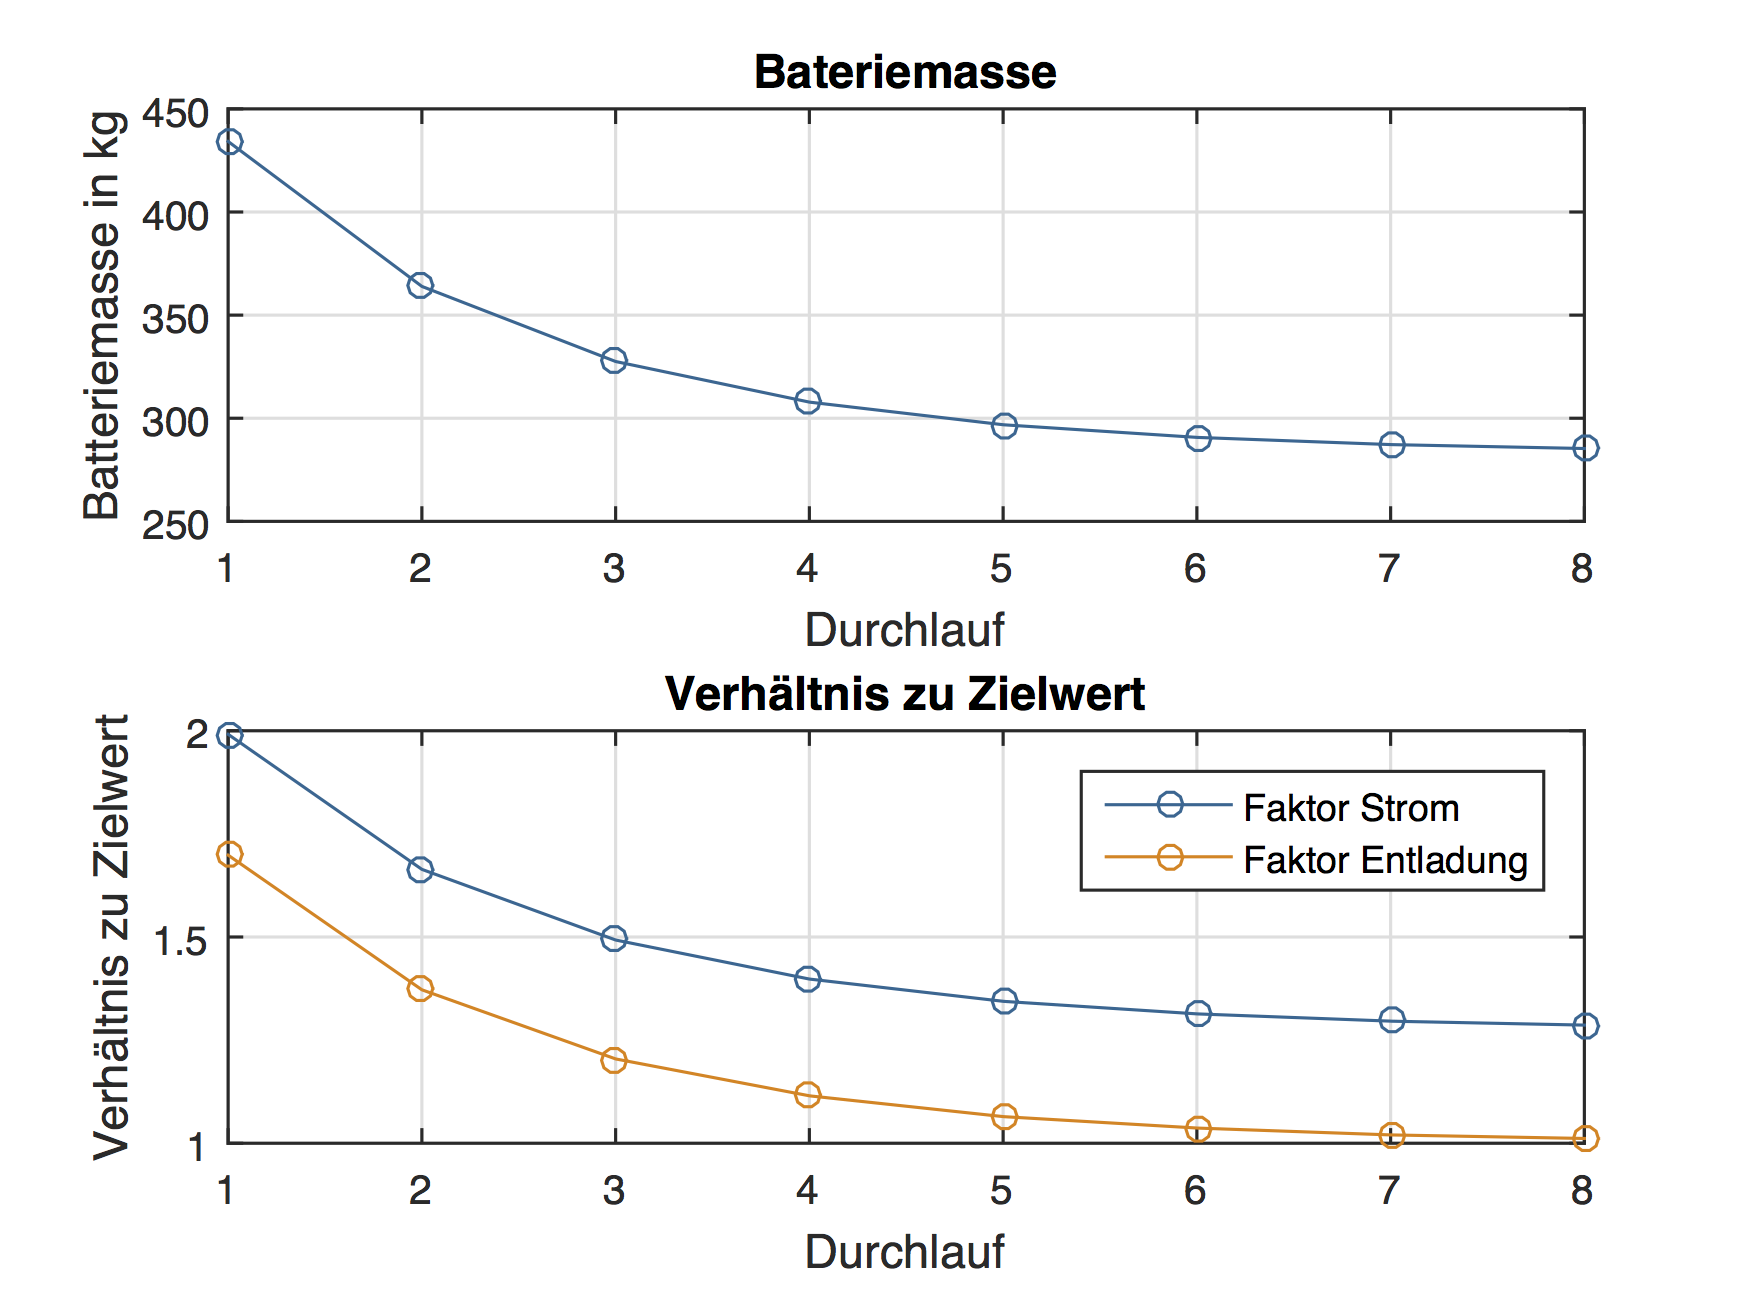
\includegraphics[width=\myFigureStandardWidth]{Optimierung}
	\caption[Optimierung der Batteriegröße]{Optimierung der Batteriegröße. Die immer langsamere Annäherung ohne Unterschreiten des Zielwertes ist gut zu erkennen. Für dieses Beispiel wurde ein Lithium-Eisenphosphat-Akku mit hoher Energie auf einem Umlauf der Linie 204 gewählt. Der Akku darf sich von 70\% Ladezustand auf minimal 30\% entladen.}
	\label{abb_Optimierung}
\end{figure}

\subsubsection{Ladesystem}
Im ursprünglichen Simulationsmodell von Götz~\cite{Gotz:2013} ist die Ladezeit durch die aufgezeichnete Strecke festgelegt und nicht variabel. Da in dieser Arbeit die Ladezeiten verschiedener Technologiekombinationen verglichen werden sollen, wurde zusätzlich ein separates Modell für den Ladevorgang erstellt. Es besteht aus dem Batteriemodell und einer Energiequelle, die nach einer Totzeit die maximale Ladeleistung bereitstellt. Die Batterie nimmt entsprechend ihrer jeweiligen Ladekurve diese Leistung teilweise oder vollständig auf. Wenn die Batterie den gewünschten Ladezustand erreicht hat, endet die Simulation und die Ergebnisse werden ausgegeben.

\subsection{Wärmeberechnung}
Der Abtransport der an der Batterie entstehenden Wärme stellt eine große Herausforderung bei der Auslegung eines Speichersystems dar. Durch Überhitzung kann die Batterie zerstört werden. Aber auch zulässige, jedoch innerhalb des Batteriepacks unterschiedliche Temperaturen führen zu einer unterschiedlichen Lebensdauer der verschiedenen Zellen und reduzieren so die Gesamtlebensdauer. Von daher wird in dieser Simulation auch die Größe des erforderlichen Kühlsystems abgeschätzt.

Wie in Abschnitt \ref{sec_waermeverluste} erläutert, überwiegt bei hohen Strömen die vom Innenwiderstand verursachte irreversible Erwärmung. Bei niedrigen Strömen ist der Anteil der reversiblen Erwärmung höher, die Gesamterwärmung jedoch niedriger. Daher wird zur Abschätzung nur der irreversible Anteil mit einem Sicherheitsfaktor von 2 verwendet. Die Erwärmung der Batterien wird mit der Batteriemasse aus dem entsprechenden Datenblatt und den von Pesaran ermittelten Wärmekapazitäten berechnet~\cite{pesaran2001battery}.

Es wird eine parallele Luftkühlung modelliert, bei der die jeweils Luft nur an einer Zelle vorbeigeführt wird. Diese Methode wird von Pesaran als einfache Möglichkeit für eine gleichmäßige Temperatur im Batteriepack empfohlen~\cite{pesaran2001battery}. Es wird angenommen, dass die Hälfte der Temperaturdifferenz zwischen Batterie und Umgebungsluft zur Kühlung verwendet werden kann. Als Umgebungstemperatur wird ein Wert von 40 $^{\circ}C$ angenommen, der noch eine kleine Reserve zur höchsten in Berlin gemessenen Temperatur von 38,1 $^{\circ}C$ bietet\cite{tempRekord}. Die benötigte Luftmenge wird durch einem PI-Regler berechnet und der Höchstwert in $\frac{g}{s}$ angegeben.

Es wird nicht unbedingt die ideale Kühlung für jede mögliche Batterie berechnet, sondern es werden vergleichbare Werte für verschiedene Batterien ermittelt, in denen Masse, Wärmekapazität und Maximaltemperatur berücksichtigt sind.

\section{Ergebnisse}
\label{simErgebnisse}
Die folgenden Ausgabedaten der Simulation wurden ausgewählt, um die Kombinationen von Lade- und Speichersystem zu vergleichen:
\begin{description}
	\item[Batteriemasse] Einheit: $kg$
	\item[Batterievolumen] Einheit: $l$
	\item[Kühlluftmasse] Einheit: $\frac{g}{s}$
	\item[Energieverbrauch] Einheit: $\frac{kWh}{km}$
	\item[Zeiteffizienz] Der Anteil der Fahrzeit an der Summe von Fahr- und Ladezeit. Zahlenwert zwischen 0 und 1, größere Werte sind besser.
	\item[Ladezyklen pro tausend Kilometer] Mit diesem Wert kann die Lebensdauer der Batterie abgeschätzt werden.\\
	Einheit: $\frac{1}{10^{3}km}$  
\end{description}

\subsection{Linie 204}
\label{erkl204} 
Bei der Ladestrategie "`Nachtladung"' fährt der Bus tagsüber ohne Zwischenladen auf der Strecke. Er absolviert 11 Touren mit einer Gesamtlänge von 141 km. Die Batterie darf sich dabei auf maximal 10\% Ladezustand entladen. Nach Betriebsschluss wird der Bus über Nacht im Depot auf 100\% Ladezustand geladen. Als Ladesystem wurde ein konduktiv-manuelles System mit 40 kW gewählt.

Bei der Ladestrategie "`Gelegenheitsladung"' wird der Bus nach jeder Folge von Hin- und Rückfahrt aufgeladen. Die Länge einer Tour beträgt 12,8 km. Beim schnellen Laden können die Ladezustände der einzelnen Zellen nicht angeglichen werden, so dass sie über den Betriebstag immer weiter divergieren. Zum Schutz gegen Tiefentladung und Überladung einzelner Zellen wird die Batterie zwischen 35\% und 65\% Ladezustand betrieben. Bei dieser Ladestrategie werden sämtliche Ladesysteme betrachtet.

Die Ergebnisse sind in Abbildung \ref{diagramme204} grafisch dargestellt und in den Tabellen \ref{204_a} bis \ref{204_e} aufgeführt.


\subsection{Linie 192}
Die Parameter sind wie in Abschnitt \ref{erkl204} gewählt, allerdings  beträgt die Länge eines Umlaufs 29,8 km. Ein Betriebstag wird zur besseren Vergleichbarkeit auch hier mit 11 Umläufen simuliert, die Gesamtlänge bei der Ladestrategie "`Nachtladung"' beträgt 217 km.

Die Ergebnisse sind in Abbildung \ref{diagramme192} grafisch dargestellt und in den Tabellen \ref{192_a} bis \ref{192_e} aufgeführt.

\begin{figure}\centering
	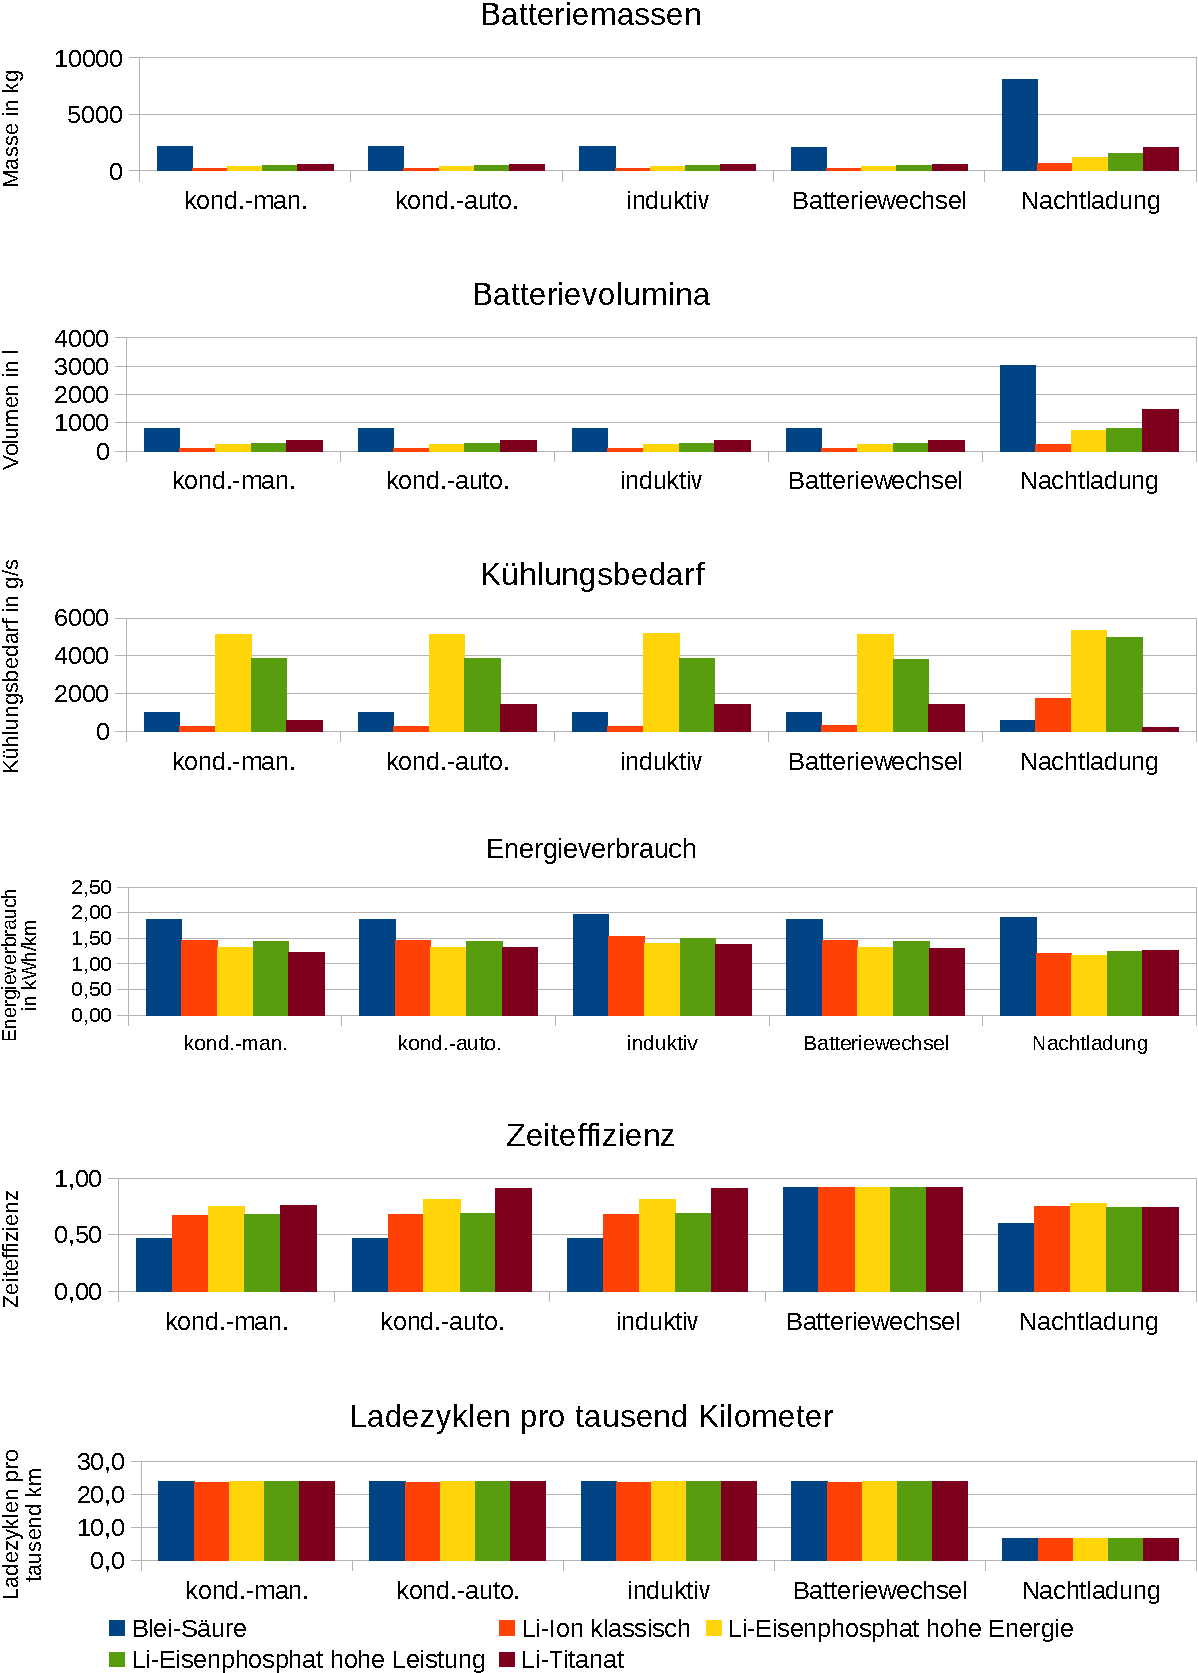
\includegraphics[height=20cm]{Diagramme204}
	\caption{Diagramme der Simulationsergebnisse für die Buslinie 204}
	\label{diagramme204}
\end{figure}

\begin{figure}\centering
	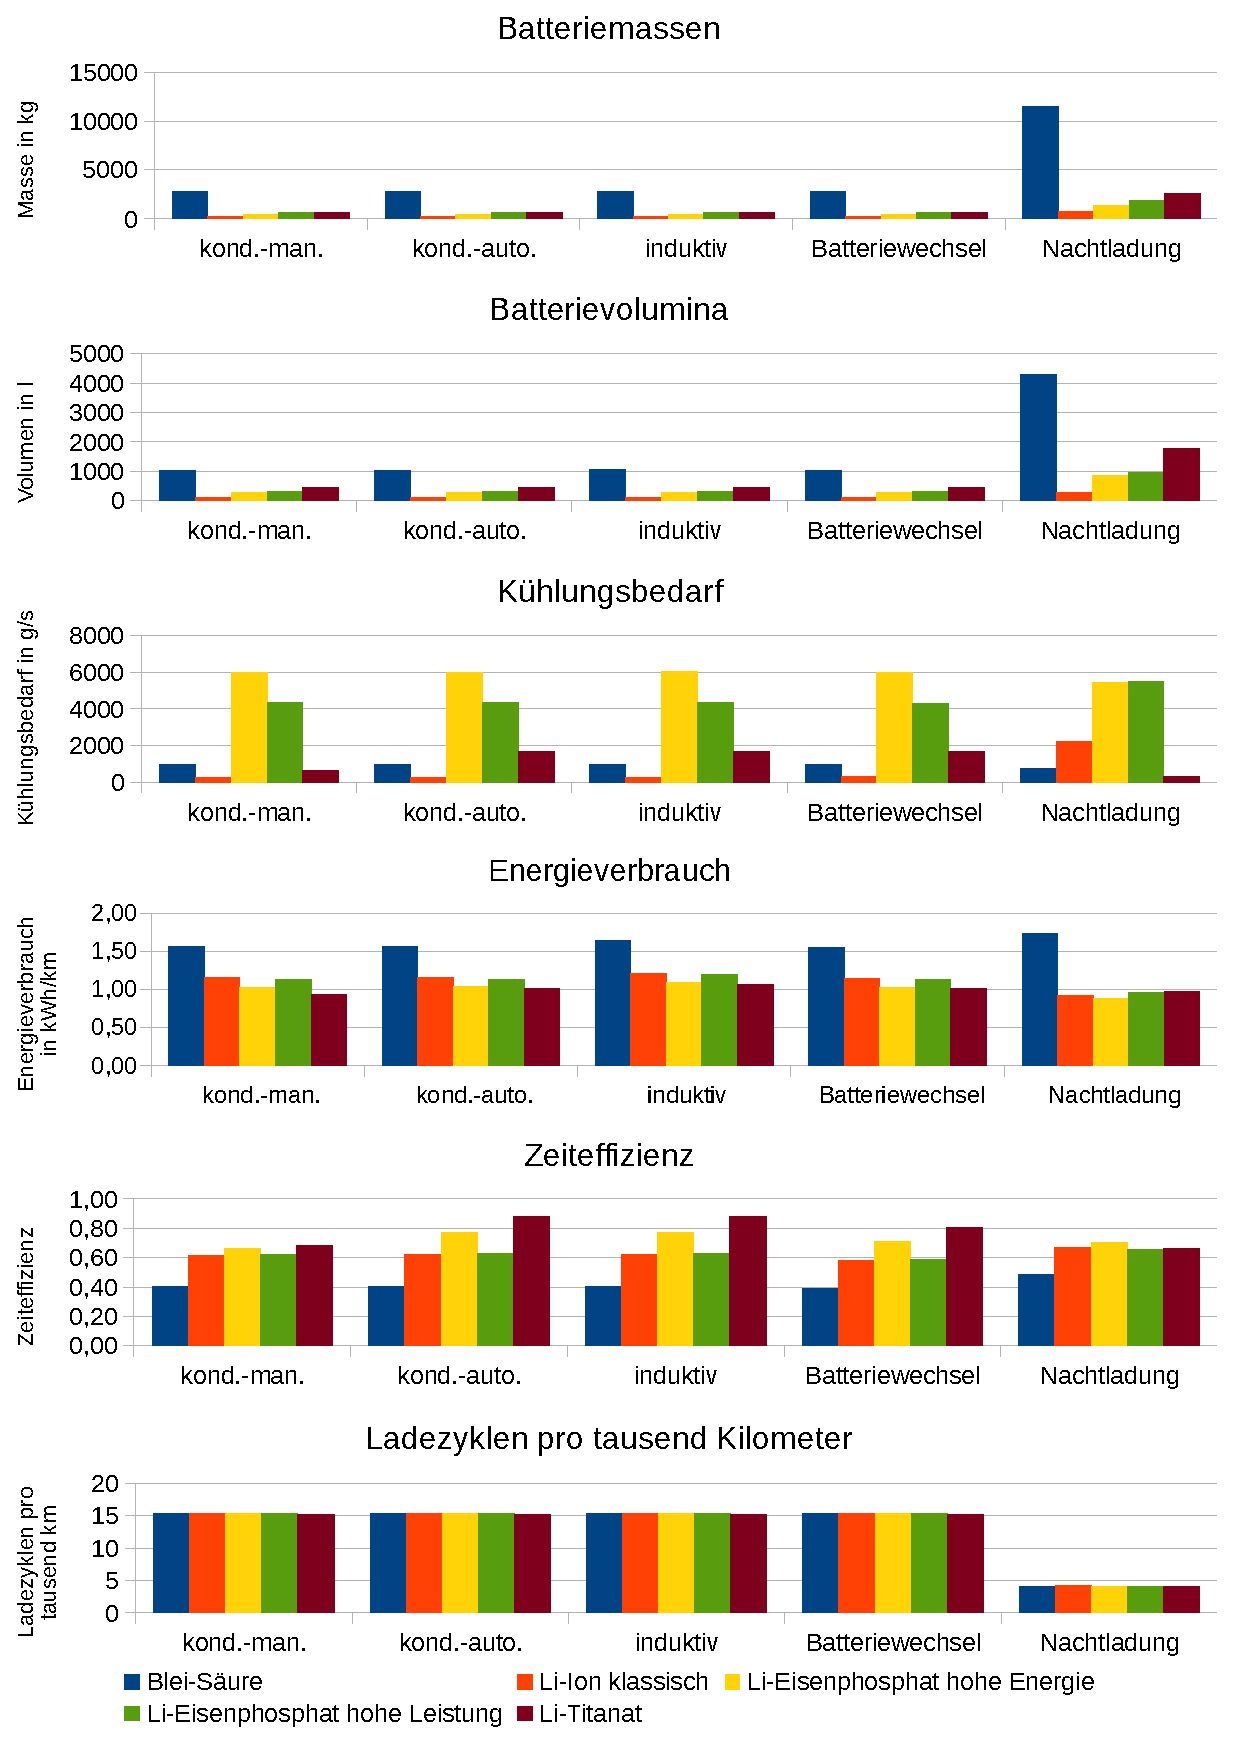
\includegraphics[height=20cm]{Diagramme192}
	\caption{Diagramme der Simulationsergebnisse für die Buslinie 192}
	\label{diagramme192}
\end{figure}

%%%%% LINIE 204 %%%%%
\begin{table}[h] \centering
	\begin{tabulary}{\linewidth}{LRRrRR}
		                                                \multicolumn{6}{c}{Batteriemassen in $kg$}                                                  \\ \toprule
		Bat./LS                          &                 \multicolumn{4}{c}{Gelegenheitsladen}                  & \multicolumn{1}{c}{Nachtladung} \\
		\cmidrule{2-5}                   & konduktiv-manuell & konduktiv-automatisch & induktiv & Batteriewechsel &               konduktiv-manuell \\ \midrule
		Blei-Säure-Batterie              &              2125 &                  2130 &     2145 &            2120 &                            8051 \\
		"`klassischer"' Li-Ionen-Akku    &               215 &                   215 &      217 &             214 &                             668 \\
		Li-Eisenphosphat (hohe Energie)  &               358 &                   359 &      361 &             357 &                            1180 \\
		Li-Eisenphosphat (hohe Leistung) &               480 &                   481 &      484 &             479 &                            1532 \\
		Lithium-Titanat                  &               540 &                   541 &      543 &             539 &                            2107 \\ \bottomrule
	\end{tabulary}
	\caption{Batteriemassen Linie 204}
	\label{204_a}
\end{table}

\begin{table} \centering
	\begin{tabulary}{\linewidth}{LRRrRR}
		                                                \multicolumn{6}{c}{Batterievolumina in $l$}                                                 \\ \toprule
		Bat./LS                          &                 \multicolumn{4}{c}{Gelegenheitsladen}                  & \multicolumn{1}{c}{Nachtladung} \\
		\cmidrule{2-5}                   & konduktiv-manuell & konduktiv-automatisch & induktiv & Batteriewechsel &               konduktiv-manuell \\ \midrule
		Blei-Säure-Batterie              &               797 &                   799 &      805 &             795 &                            3020 \\
		"`klassischer"' Li-Ionen-Akku    &                78 &                    78 &       78 &              78 &                             242 \\
		Li-Eisenphosphat (hohe Energie)  &               217 &                   217 &      219 &             217 &                             715 \\
		Li-Eisenphosphat (hohe Leistung) &               251 &                   251 &      253 &             250 &                             800 \\
		Lithium-Titanat                  &               378 &                   379 &      380 &             377 &                            1475 \\ \bottomrule
	\end{tabulary}
	\caption{Batterievolumina Linie 204}
\end{table}

\begin{table} \centering
	\begin{tabulary}{\linewidth}{LRRrRR}
		                                              \multicolumn{6}{c}{Kühlbedarf in $\frac{g}{s}$}                                               \\ \toprule
		Bat./LS                          &                 \multicolumn{4}{c}{Gelegenheitsladen}                  & \multicolumn{1}{c}{Nachtladung} \\
		\cmidrule{2-5}                   & konduktiv-manuell & konduktiv-automatisch & induktiv & Batteriewechsel &               konduktiv-manuell \\ \midrule
		Blei-Säure-Batterie              &               969 &                   972 &      980 &             966 &                             577 \\
		"`klassischer"' Li-Ionen-Akku    &               245 &                   241 &      242 &             276 &                            1735 \\
		Li-Eisenphosphat (hohe Energie)  &              5130 &                  5141 &     5174 &            5119 &                            5331 \\
		Li-Eisenphosphat (hohe Leistung) &              3827 &                  3835 &     3858 &            3820 &                            4989 \\
		Lithium-Titanat                  &               582 &                  1421 &     1426 &            1417 &                             202 \\ \bottomrule
	\end{tabulary}
	\caption{Kühlungsbedarf Linie 204}
\end{table}

\begin{table} \centering
	\begin{tabulary}{\linewidth}{LRRrRR}
		                                         \multicolumn{6}{c}{Energieverbrauch in $\frac{kWh}{km}$}                                           \\ \toprule
		Bat./LS                          &                 \multicolumn{4}{c}{Gelegenheitsladen}                  & \multicolumn{1}{c}{Nachtladung} \\
		\cmidrule{2-5}                   & konduktiv-manuell & konduktiv-automatisch & induktiv & Batteriewechsel &               konduktiv-manuell \\ \midrule
		Blei-Säure-Batterie              &              1,87 &                  1,88 &     1,97 &            1,87 &                            1,91 \\
		"`klassischer"' Li-Ionen-Akku    &              1,45 &                  1,46 &     1,53 &            1,45 &                            1,21 \\
		Li-Eisenphosphat (hohe Energie)  &              1,31 &                  1,33 &     1,39 &            1,32 &                            1,16 \\
		Li-Eisenphosphat (hohe Leistung) &              1,43 &                  1,43 &     1,50 &            1,43 &                            1,24 \\
		Lithium-Titanat                  &              1,22 &                  1,31 &     1,37 &            1,31 &                            1,26 \\ \bottomrule
	\end{tabulary}
	\caption{Energieverbrauch Linie 204}
\end{table}

\begin{table} \centering
	\begin{tabulary}{\linewidth}{LRRrRR}
		                                                     \multicolumn{6}{c}{Zeiteffizienz}                                                      \\ \toprule
		Bat./LS                          &                 \multicolumn{4}{c}{Gelegenheitsladen}                  & \multicolumn{1}{c}{Nachtladung} \\
		\cmidrule{2-5}                   & konduktiv-manuell & konduktiv-automatisch & induktiv & Batteriewechsel &               konduktiv-manuell \\ \midrule
		Blei-Säure-Batterie              &              0,46 &                  0,46 &     0,46 &            0,92 &                            0,60 \\
		"`klassischer"' Li-Ionen-Akku    &              0,67 &                  0,67 &     0,67 &            0,92 &                            0,75 \\
		Li-Eisenphosphat (hohe Energie)  &              0,75 &                  0,81 &     0,81 &            0,92 &                            0,78 \\
		Li-Eisenphosphat (hohe Leistung) &              0,68 &                  0,68 &     0,68 &            0,92 &                            0,74 \\
		Lithium-Titanat                  &              0,76 &                  0,90 &     0,90 &            0,92 &                            0,74 \\ \bottomrule
	\end{tabulary}
	\caption{Zeiteffizienz (Anteil Fahrzeit an Gesamtzeit) Linie 204}
\end{table}

\begin{table} \centering
	\begin{tabulary}{\linewidth}{LRRrRR}
		                                           \multicolumn{6}{c}{Ladezyklen pro tausend Kilometer}                                             \\ \toprule
		Bat./LS                          &                 \multicolumn{4}{c}{Gelegenheitsladen}                  & \multicolumn{1}{c}{Nachtladung} \\
		\cmidrule{2-5}                   & konduktiv-manuell & konduktiv-automatisch & induktiv & Batteriewechsel &               konduktiv-manuell \\ \midrule
		Blei-Säure-Batterie              &                24 &                    24 &       24 &              24 &                               6 \\
		"`klassischer"' Li-Ionen-Akku    &                24 &                    24 &       24 &              24 &                               6 \\
		Li-Eisenphosphat (hohe Energie)  &                24 &                    24 &       24 &              24 &                               6 \\
		Li-Eisenphosphat (hohe Leistung) &                24 &                    24 &       24 &              24 &                               6 \\
		Lithium-Titanat                  &                24 &                    24 &       24 &              24 &                               6 \\ \bottomrule
	\end{tabulary}
	\caption{Ladezyklen pro tausend Kilometer Linie 204}
	\label{204_e}
\end{table}

%%%%% LINIE 192 %%%%%
\begin{table} \centering
	\begin{tabulary}{\linewidth}{LRRrRR}
		                                                \multicolumn{6}{c}{Batteriemassen in $kg$}                                                  \\ \toprule
		Bat./LS                          &                 \multicolumn{4}{c}{Gelegenheitsladen}                  & \multicolumn{1}{c}{Nachtladung} \\
		\cmidrule{2-5}                   & konduktiv-manuell & konduktiv-automatisch & induktiv & Batteriewechsel &               konduktiv-manuell \\ \midrule
		Blei-Säure-Batterie              &              2751 &                  2759 &     2781 &            2744 &                           11432 \\
		"`klassischer"' Li-Ionen-Akku    &               264 &                   265 &      267 &             264 &                             797 \\
		Li-Eisenphosphat (hohe Energie)  &               435 &                   436 &      439 &             434 &                            1400 \\
		Li-Eisenphosphat (hohe Leistung) &               592 &                   594 &      598 &             591 &                            1851 \\
		Lithium-Titanat                  &               647 &                   648 &      652 &             646 &                            2559 \\ \bottomrule
	\end{tabulary}
	\caption{Batteriemassen Linie 192}
	\label{192_a}
\end{table}

\begin{table} \centering
	\begin{tabulary}{\linewidth}{LRRrRR}
		                                                \multicolumn{6}{c}{Batterievolumina in $l$}                                                 \\ \toprule
		Bat./LS                          &                 \multicolumn{4}{c}{Gelegenheitsladen}                  & \multicolumn{1}{c}{Nachtladung} \\
		\cmidrule{2-5}                   & konduktiv-manuell & konduktiv-automatisch & induktiv & Batteriewechsel &               konduktiv-manuell \\ \midrule
		Blei-Säure-Batterie              &              1032 &                  1035 &     1043 &            1029 &                            4288 \\
		"`klassischer"' Li-Ionen-Akku    &                96 &                    96 &       97 &              95 &                             288 \\
		Li-Eisenphosphat (hohe Energie)  &               264 &                   264 &      266 &             263 &                             849 \\
		Li-Eisenphosphat (hohe Leistung) &               309 &                   310 &      313 &             309 &                             966 \\
		Lithium-Titanat                  &               453 &                   454 &      456 &             452 &                            1791 \\ \bottomrule
	\end{tabulary}
	\caption{Batterievolumina Linie 192}
\end{table}

\begin{table} \centering
	\begin{tabulary}{\linewidth}{LRRrRR}
		                                              \multicolumn{6}{c}{Kühlbedarf in $\frac{g}{s}$}                                               \\ \toprule
		Bat./LS                          &                 \multicolumn{4}{c}{Gelegenheitsladen}                  & \multicolumn{1}{c}{Nachtladung} \\
		\cmidrule{2-5}                   & konduktiv-manuell & konduktiv-automatisch & induktiv & Batteriewechsel &               konduktiv-manuell \\ \midrule
		Blei-Säure-Batterie              &               967 &                   971 &      981 &             964 &                             770 \\
		"`klassischer"' Li-Ionen-Akku    &               269 &                   264 &      265 &             303 &                            2241 \\
		Li-Eisenphosphat (hohe Energie)  &              5972 &                  5985 &     6022 &            5960 &                            5461 \\
		Li-Eisenphosphat (hohe Leistung) &              4321 &                  4329 &     4354 &            4313 &                            5512 \\
		Lithium-Titanat                  &               625 &                  1687 &     1694 &            1683 &                             306 \\ \bottomrule
	\end{tabulary}
	\caption{Kühlungsbedarf Linie 192}
\end{table}

\begin{table} \centering
	\begin{tabulary}{\linewidth}{LRRrRR}
		                                         \multicolumn{6}{c}{Energieverbrauch in $\frac{kWh}{km}$}                                           \\ \toprule
		Bat./LS                          &                 \multicolumn{4}{c}{Gelegenheitsladen}                  & \multicolumn{1}{c}{Nachtladung} \\
		\cmidrule{2-5}                   & konduktiv-manuell & konduktiv-automatisch & induktiv & Batteriewechsel &               konduktiv-manuell \\ \midrule
		Blei-Säure-Batterie              &              1,56 &                  1,56 &     1,64 &            1,56 &                            1,74 \\
		"`klassischer"' Li-Ionen-Akku    &              1,16 &                  1,16 &     1,22 &            1,15 &                            0,93 \\
		Li-Eisenphosphat (hohe Energie)  &              1,02 &                  1,04 &     1,09 &            1,03 &                            0,88 \\
		Li-Eisenphosphat (hohe Leistung) &              1,14 &                  1,14 &     1,20 &            1,13 &                            0,96 \\
		Lithium-Titanat                  &              0,94 &                  1,01 &     1,06 &            1,01 &                            0,98 \\ \bottomrule
	\end{tabulary}
	\caption{Energieverbrauch Linie 1929}
\end{table}

\begin{table} \centering
	\begin{tabulary}{\linewidth}{LRRrRR}
		                                                     \multicolumn{6}{c}{Zeiteffizienz}                                                      \\ \toprule
		Bat./LS                          &                 \multicolumn{4}{c}{Gelegenheitsladen}                  & \multicolumn{1}{c}{Nachtladung} \\
		\cmidrule{2-5}                   & konduktiv-manuell & konduktiv-automatisch & induktiv & Batteriewechsel &               konduktiv-manuell \\ \midrule
		Blei-Säure-Batterie              &              0,40 &                  0,41 &     0,41 &            0,90 &                            0,49 \\
		"`klassischer"' Li-Ionen-Akku    &              0,61 &                  0,62 &     0,62 &            0,90 &                            0,67 \\
		Li-Eisenphosphat (hohe Energie)  &              0,66 &                  0,77 &     0,77 &            0,90 &                            0,70 \\
		Li-Eisenphosphat (hohe Leistung) &              0,62 &                  0,63 &     0,63 &            0,90 &                            0,66 \\
		Lithium-Titanat                  &              0,68 &                  0,88 &     0,88 &            0,90 &                            0,67 \\ \bottomrule
	\end{tabulary}
	\caption{Zeiteffizienz (Anteil Fahrzeit an Gesamtzeit) Linie 192}
\end{table}

\begin{table} \centering
	\begin{tabulary}{\linewidth}{LRRrRR}
		                                           \multicolumn{6}{c}{Ladezyklen pro tausend Kilometer}                                             \\ \toprule
		Bat./LS                          &                 \multicolumn{4}{c}{Gelegenheitsladen}                  & \multicolumn{1}{c}{Nachtladung} \\
		\cmidrule{2-5}                   & konduktiv-manuell & konduktiv-automatisch & induktiv & Batteriewechsel &               konduktiv-manuell \\ \midrule
		Blei-Säure-Batterie              &                15 &                    15 &       15 &               4 &  \\
		"`klassischer"' Li-Ionen-Akku    &                15 &                    15 &       15 &               4 &  \\
		Li-Eisenphosphat (hohe Energie)  &                15 &                    15 &       15 &               4 &  \\
		Li-Eisenphosphat (hohe Leistung) &                15 &                    15 &       15 &               4 &  \\
		Lithium-Titanat                  &                15 &                    15 &       51 &               4 &  \\ \bottomrule
	\end{tabulary}
	\caption{Ladezyklen pro tausend Kilometer Linie 192}
	\label{192_e}
\end{table}